\documentclass[11pt]{article}
\usepackage[utf8]{inputenc}
\usepackage[top=60pt, bottom=60pt, left=70pt, right=70pt]{geometry}
\usepackage{graphicx}
% Default fixed font does not support bold face
\DeclareFixedFont{\ttb}{T1}{txtt}{bx}{n}{8} % for bold
\DeclareFixedFont{\ttm}{T1}{txtt}{m}{n}{8}  % for normal

% Custom colors
\usepackage{color}
\definecolor{deepblue}{rgb}{0,0,0.5}
\definecolor{deepred}{rgb}{0.6,0,0}
\definecolor{deepgreen}{rgb}{0,0.5,0}
\definecolor{commentgrey}{rgb}{0.5,0.5,0.5}
\usepackage{listings}

% Python style for highlighting
\lstset{
language=Python,
basicstyle=\ttm,
otherkeywords={self},             % Add keywords here
keywordstyle=\ttb\color{deepblue},
emph={MyClass,__init__},          % Custom highlighting
emphstyle=\ttb\color{deepred},    % Custom highlighting style
stringstyle=\color{deepgreen},
frame=tb,                         % Any extra options here
commentstyle=\color{commentsgrey}
}


\title{ICSolar Model}
\author{Daniel W. Zaide}

\begin{document}

\maketitle
Consider the model of air and water interaction consisting of an initial inlet region (denoted by 0) and a pair of regions, an open region with pipe followed by a module, denoted by (1,2) satisfying 
\begin{eqnarray} 
W_1: & & \dot{m}_wC_{p,w}(T_{w,1}-T_{w,0}) - h_{wa}(T_{a,1}-T_{w,1}) = 0 \\
A_1: & & \dot{m}_aC_{p,a}(T_{a,1}-T_{a,0}) - h_{wa}(T_{w,1}-T_{a,1}) - h_{e}(T_e-T_{a,1}) - h_{i}(T_i-T_{a,1})= 0 \\
W_2: & & \dot{m}_wC_{p,w}(T_{w,2}-T_{w,1}) - Q_w = 0\\
A_2: & & \dot{m}_aC_{p,a}(T_{a,2}-T_{a,1}) - Q_a = 0 
\end{eqnarray}
Where $i$ and $e$ are interior and exterior contributions. Each pair of these forms a `module'. In this work, we use
\begin{eqnarray}
C_{p,w} & = & 4.218 kJ/(kg K) \\
\dot{m}_w & = & 0.0008483 kg/s \\
C_{p,a} & = & 1.005 kJ/(kg K) \\
\dot{m}_a & = & 0.384 kg/s \\
h_{wa} & = & 4.823 \times 10^{-5} kW/(K m)\\
h_{i} & = & 1.572 \times 10^{-4} kW/(K m)\\
h_{e} & = & 4.837 \times 10^{-4} kW/(K m)\\
\end{eqnarray}
With Initial and Boundary Conditions of $T_{a,0} = 20 C, T_i = 25.0 C, T_e = 22.5 C$. At this point, we set $Q_a = 0$ as the surrounding air acts like a reservoir and its effect is currently minimal. Our inputs are $T_{w,0}$ and $Q_w$ from experimental data. We take experimental data from the file \texttt{nov25\_2.csv} located in the github repository. 

\begin{figure}[!ht]
\centering
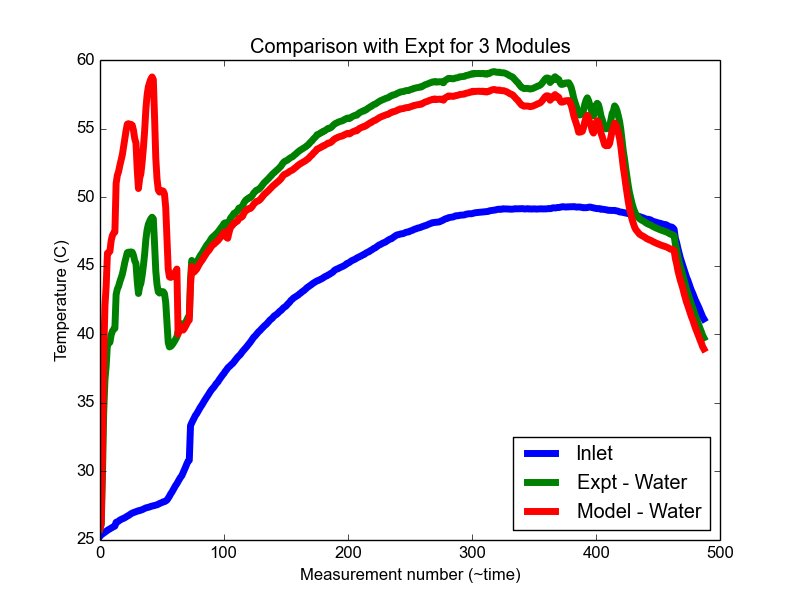
\includegraphics[width=0.6\textwidth]{nov25.png}
\caption{Comparison between experiment and model for 3 modules, water temperature in last module compared.}
\end{figure}
\begin{figure}[!ht]
\centering
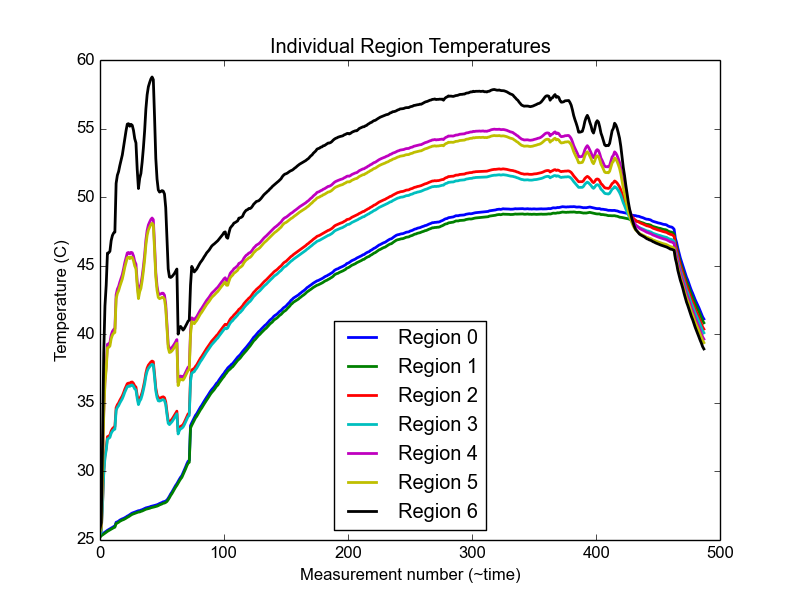
\includegraphics[width=0.6\textwidth]{nov25modules.png}
\caption{Model results for 3 module case, using experimental inputs. Regions 2,4,6 correspond to modules.}
\end{figure}

\begin{figure}[!ht]
\centering
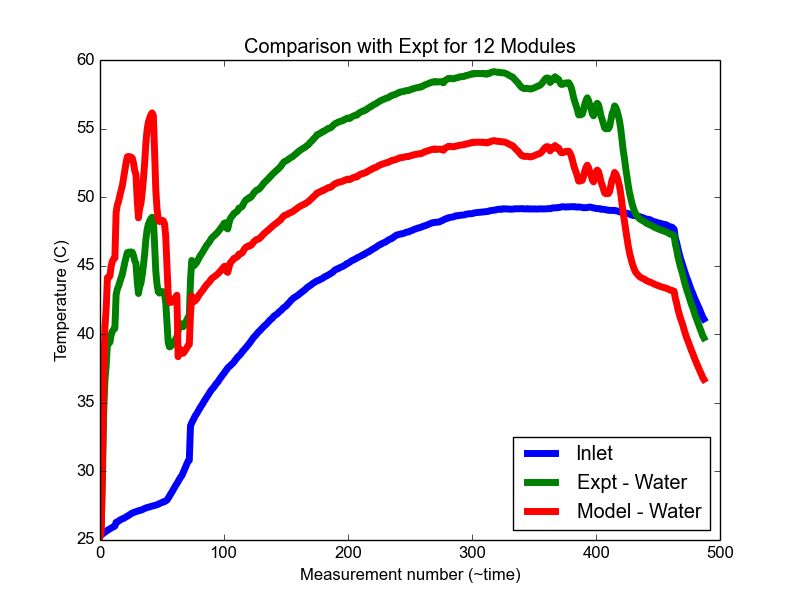
\includegraphics[width=0.6\textwidth]{nov25_12.png}
\caption{Comparison between experiment (3 modules) and model (12 modules), water temperature in last module compared.}
\end{figure}
\begin{figure}[!ht]
\centering
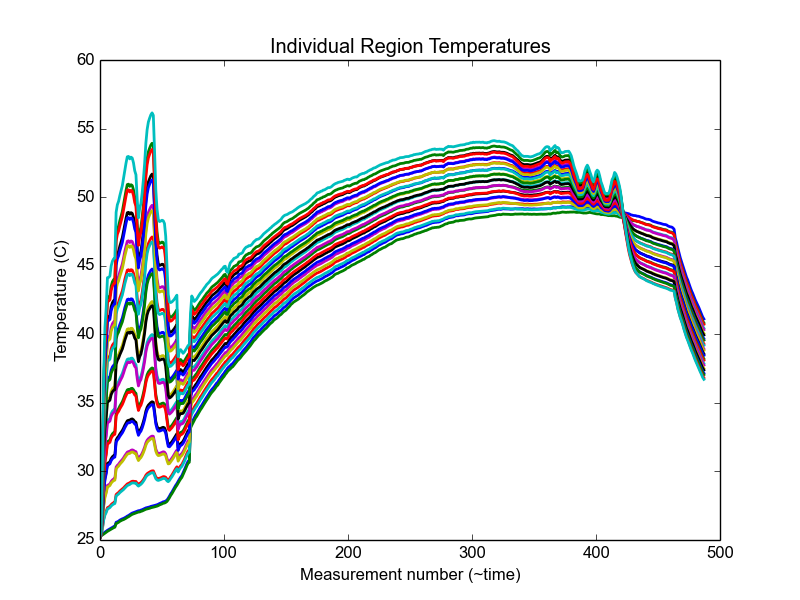
\includegraphics[width=0.6\textwidth]{nov25modules_12.png}
\caption{Model results for 3 module case, using experimental inputs. Legend not shown, but self explanatory.}
\end{figure}

\end{document}

% \section{``In-text'' listing highlighting}

% \begin{lstlisting}
% class MyClass(Yourclass):
%     def __init__(self, my, yours):
%         bla = '5 1 2 3 4'
%         print bla
% \end{lstlisting}

% \section{External listing highlighting}

% \lstinputlisting{../ICSolar.py}

% \section{Inline highlighting}

% Definition \lstinline{class MyClass} means \dots